\documentclass[xcolor=dvipsnames]{beamer}
\usepackage[english]{babel}
\usepackage[latin1]{inputenc}
\usepackage{times}
\usepackage[T1]{fontenc}
\usepackage{graphicx}
\usepackage[absolute, overlay]{textpos}
\usepackage{tikz}
\usepackage{multimedia}
\usepackage{soul}
\usepackage{wasysym}
\def\urltilda{\kern -.15em\lower .7ex\hbox{\~{}}\kern .04em}
\def\deg{^{\circ}}

\setlength{\TPHorizModule}{0.01\textwidth}
\setlength{\TPVertModule}{\TPHorizModule}
\definecolor{darkyellow}{rgb}{1,0.75,0}
\definecolor{black}{rgb}{0,0,0}
\definecolor{skyblue}{rgb}{0.7,0.8,1.0}
\definecolor{black}{rgb}{0,0,0}
\definecolor{darkgrey}{rgb}{0.3,0.3,0.3}
\definecolor{medgrey}{rgb}{0.5,0.5,0.5}
\definecolor{lightgrey}{rgb}{0.8,0.8,0.8}
\definecolor{lightMahogany}{rgb}{0.9,0.8,0.8}
\definecolor{darkblue}{rgb}{0,0,0.5}
\definecolor{darkgreen}{rgb}{0.1,0,0.3}
\definecolor{darkred}{rgb}{0.6,0,0}

\newcommand{\params}{\Xi}
\newcommand{\Eobsi}{E'_i}
\newcommand{\phiobsi}{\phi'_i}
\newcommand{\Etruei}{E_i}
\newcommand{\phitruei}{\phi_{i}}
\newcommand{\Eobsij}{E'_{ij}}
\newcommand{\phiobsij}{\phi'_{ij}}
\newcommand{\Etrueij}{E_{ij}}
\newcommand{\phitrueij}{\phi_{ij}}
\newcommand{\obs}{\mathrm{obs}}
\newcommand{\true}{\mathrm{true}}
\newcommand{\Like}{\mathcal{L}}
\newcommand{\ntot}{{n_\mathrm{tot}}}
\newcommand{\ntotj}{{n_{\mathrm{tot},j}}}
\newcommand{\diff}{\mathrm{d}}
\newcommand{\cblue}[1]{{\color[rgb]{0.1, 0.0, 0.6} #1}}
\newcommand{\cgreen}[1]{{\color[rgb]{0.0, 0.6, 0.1} #1}}
\newcommand{\corange}[1]{{\color[rgb]{0.9, 0.5, 0.0} #1}}
\newcommand{\cbluewhen}[2]{{\color#2[rgb]{0.1, 0.0, 0.6} #1}}
\newcommand{\cgreenwhen}[2]{{\color#2[rgb]{0.0, 0.6, 0.1} #1}}
\newcommand{\corangewhen}[2]{{\color#2[rgb]{0.9, 0.5, 0.0} #1}}

\newcommand{\manual}[1]{
  \begin{tikzpicture}[x=\textwidth, y=0.82\textheight]%, >=angle 90]
    \useasboundingbox (0, 0) rectangle (1, 1);
    #1
  \end{tikzpicture}
}

%%% Custom nodes.

\newcommand{\basenode}[4]{
  \node[outer sep=6pt, anchor=#3] (#1) at (#2){#4};
}

\newcommand{\emptynode}[2]{
  \basenode{#1}{#2}{base}{}

}

\newcommand{\minipagenode}[5]{
  \basenode{#1}{#2}{#3}{
    \begin{minipage}{#4}
      \vspace*{-12pt}
      {#5}
      \vspace*{-8pt}
  \end{minipage}}

}

\newcommand{\imagenode}[5]{
  \minipagenode{#1}{#2}{#3}{#4}{%
    \includegraphics[width=\textwidth]{#5}%
  }
}

%%% Connectors.

\newcommand{\connect}[4]{%
  \draw[<->, color=darkpurple, line width=1pt, out=#3, in=#4] (#1) to (#2);
}
\newcommand{\connectcolor}[5]{%
  \draw[<->, color=#5, line width=1pt, out=#3, in=#4] (#1) to (#2);
}
\newcommand{\hconnect}[3]{%
  \draw[<->, color=darkpurple, line width=1pt]
  (#1.east) .. controls +(right:#3) and +(left:#3) .. (#2.west);
}
\newcommand{\vconnect}[3]{%
  \draw[<->, color=darkpurple, line width=1pt]
  (#1.south) .. controls +(down:#3) and +(up:#3) .. (#2.north);
}

\newenvironment{litemize}
{\usebeamercolor[fg]{item color}%
\scriptsize\begin{list}{$\bullet$}{%
\setlength{\itemindent}{0pt}%
\setlength{\labelwidth}{10pt}%
\setlength{\leftmargin}{15pt}%
}}
{\end{list}}

\mode<presentation>
{
  \usetheme{Warsaw}
  \usecolortheme[named=Mahogany]{structure}
  \setbeamercovered{transparent}
  \setbeamercolor*{section in toc}{bg=white, fg=Mahogany}
}

%\beamerdefaultoverlayspecification{<+->}

\AtBeginSubsection[]
{
  \begin{frame}<beamer>
    \frametitle{Outline}
  \begin{columns}[t]
\column{0.8\textwidth}
\tableofcontents[sections={1-3}, currentsection, currentsubsection]
  \end{columns}
  \end{frame}
}

\AtBeginSection[]
{
  \begin{frame}<beamer>
    \frametitle{Outline}
  \begin{columns}[t]
\column{0.8\textwidth}
\tableofcontents[sections={1-3}, currentsection, currentsubsection]
  \end{columns}
  \end{frame}
}

\setbeamertemplate{subsection in head/foot shaded}
{\textcolor{structure!70!white}{\insertsubsectionhead}}
\setbeamertemplate{subsection in head/foot}{\textcolor{white}\insertsubsectionhead}

\title[{\textcolor{white}Including astroparticle data in global fits for new physics}]{\textcolor{white}{Getting serious about including astroparticle data in global fits to new physics scenarios}}
\author[\textcolor{medgrey}{Pat Scott -- Feb 27 -- UC Irvine Joint Particle Seminar}]{Pat Scott}
\institute{\small{Department of Physics, McGill University}}
\date[Feb 27 2013]{Slides available from \color[rgb]{0.1, 0.2, 0.6} \href{http://www.physics.mcgill.ca/~patscott}{\tt http://www.physics.mcgill.ca/{\urltilda}patscott}}
\pgfdeclareimage[height=0.7cm]{university-logo}{McGill_crest}
\logo{\pgfuseimage{university-logo}}

\subject{Talks}

\begin{document}

\begin{frame}
  \titlepage
\end{frame}

\begin{frame}<beamer>
  \frametitle{Outline}
\begin{columns}[t]
  \column{0.8\textwidth}
  \tableofcontents[sections={1-3}]
\end{columns}
\end{frame}

\section{The Problem}

\begin{frame}
\frametitle{Searching for new physics}

\cblue{Many reasons to look for physics Beyond the Standard Model (BSM):}
\begin{itemize}
\item Higgs mass (hierarchy problem $+$ vacuum stability)
\item Dark matter exists
\item Baryon asymmetry
\item Neutrino masses and mixings
\end{itemize}

\visible<2->{
\cblue{So what do we do about it?}
\begin{itemize}
\item \cgreenwhen{Make new particles at high-$E$ colliders}{<4>}
\item \cgreenwhen{Study rare processes at high-$L$ colliders}{<4>}
\item \alert<3>{\cgreenwhen{Hunt for dark matter}{<4>}}
\item Look for kooky neutrino physics
\end{itemize}
}

\end{frame}


\subsection{Beyond the SM with astroparticle probes}

\begin{frame}
\frametitle{Dark matter searches}

  \begin{itemize}
  \item
  {Direct detection -- nuclear collisions and recoils -- CDMS, XENON, DAMA, CRESST, CoGeNT, etc}
  \item
  {\visible<5->{Direct production -- missing $E_\mathrm{T}$ or otherwise -- LHC, Tevatron}}
  \item
  \visible<7->{Indirect detection -- annihilations producing
  \begin{itemize}
    \footnotesize
    \item{\alert<10>{gamma-rays -- \emph{Fermi}, HESS, CTA}}
    \item{anti-protons -- PAMELA, AMS}
    \item{anti-deuterons -- GAPS}
    \item{\alert<10>{neutrinos -- IceCube}, ANTARES}
    \item{$e^+e^-$ -- PAMELA, \emph{Fermi}, ATIC, AMS}\\
    {$\rightarrow$ secondary radiation: Compton$^{-1}$,\\synchrotron, bremsstrahlung}
    \item{\alert<10>{secondary impacts on the CMB}}
  \end{itemize}}
  \item
  \visible<9->{{Dark stars -- JWST, VLT}}
  \end{itemize}
  
  \begin{textblock}{70}(40,40)
    \only<2>{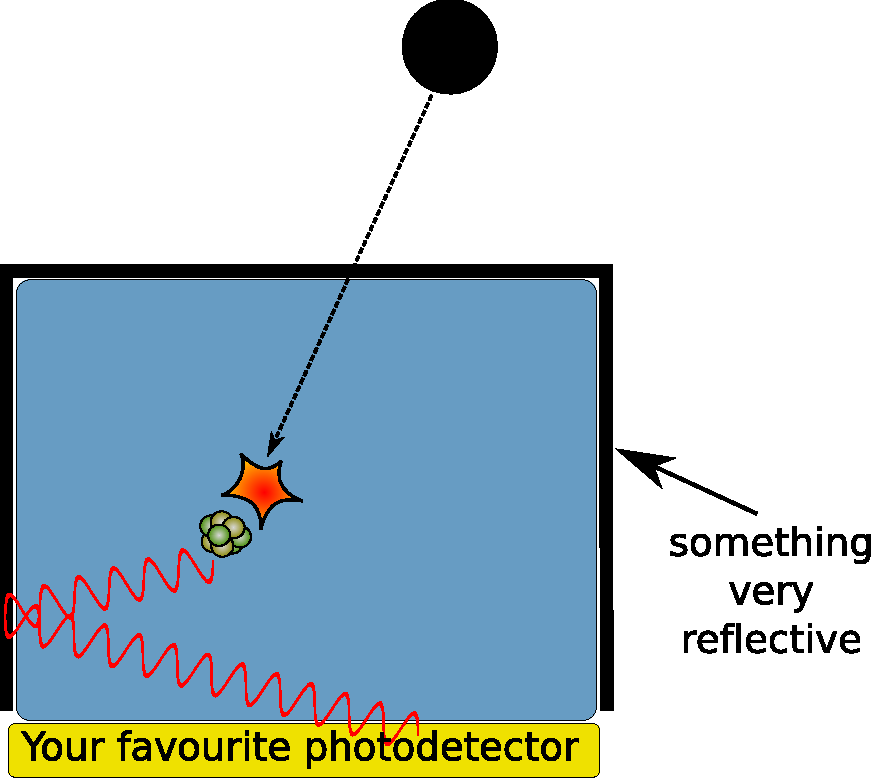
\includegraphics[width=0.6\linewidth]{SolidScintillator}}
  \end{textblock}

  \begin{textblock}{80}(25,40)
    \only<3>{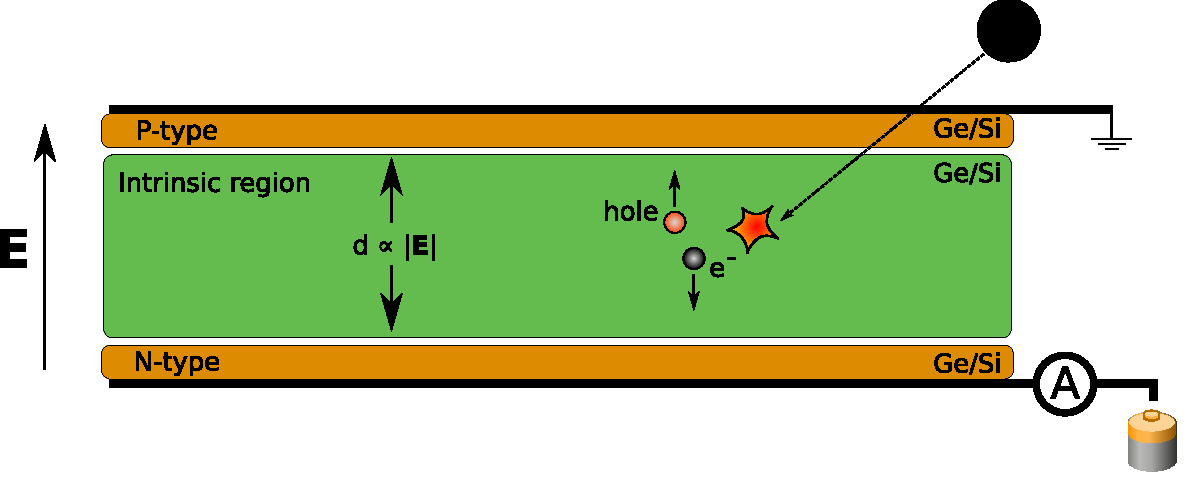
\includegraphics[width=\linewidth]{IonisationDetector}}
  \end{textblock}

  \begin{textblock}{60}(60,31)
    \only<4>{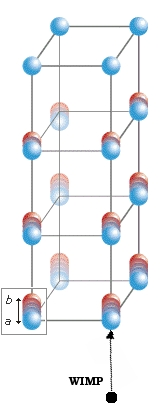
\includegraphics[width=0.35\linewidth]{Phonons}}
  \end{textblock}

  \begin{textblock}{65}(32,32)
    \only<6>{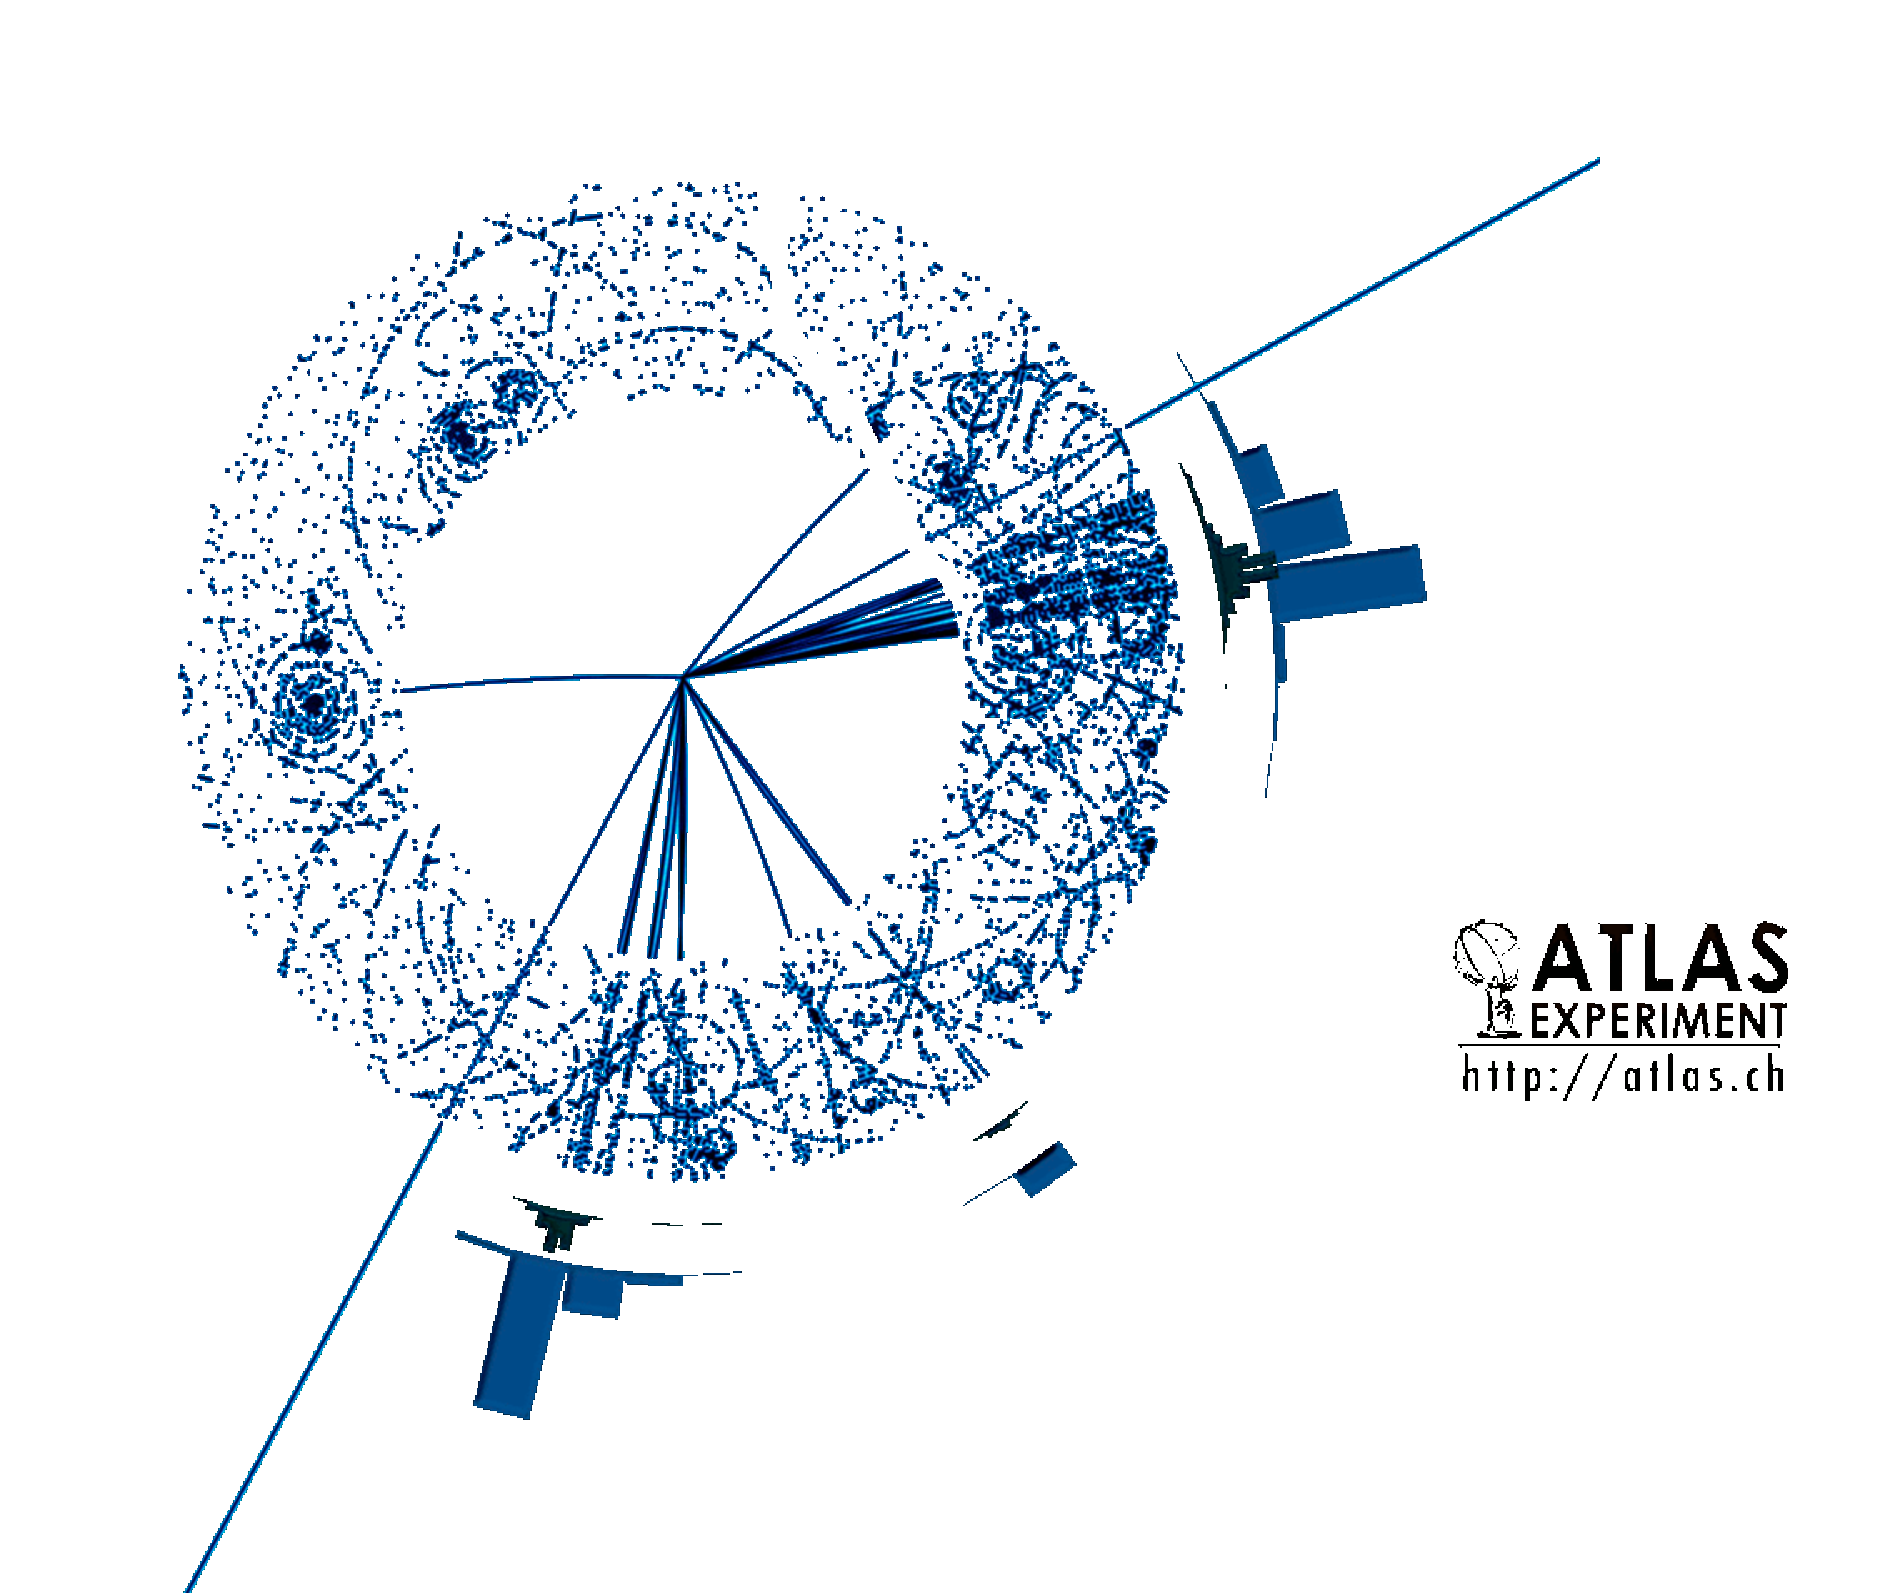
\includegraphics[width=\linewidth]{susy_sim3}}
  \end{textblock}

  \begin{textblock}{40}(75,44)
    \only<8->{\hspace{10mm}{\tiny(Weniger \textit{JCAP}, 1204.2797)}
    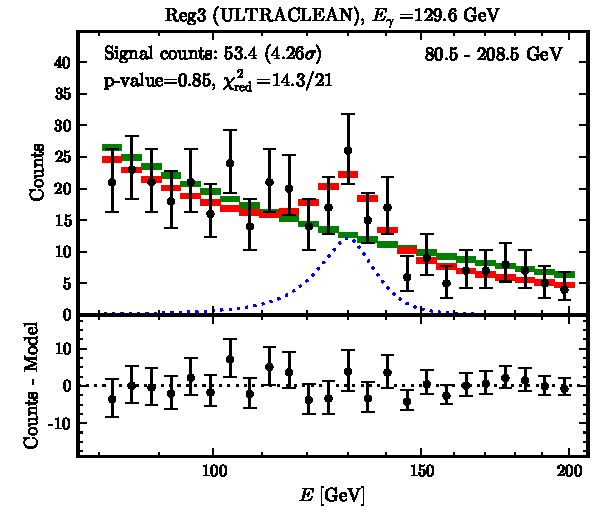
\includegraphics[width=\linewidth]{line}}
  \end{textblock}

\end{frame}


\begin{frame}
\frametitle{``The rest''}

In order of (my own completely biased opinion of) usefulness for probing BSM physics:

\begin{enumerate}
\item{\cblue{Neutrino physics (cosmological, solar, atmospheric)} \\\hspace{3mm}\footnotesize Masses, mixings, additional sterile neutrinos\\\hspace{3mm}Mass-generation models often require RH $\nu$, extra symmetry groups}
\item{\cblue{BBN} \\\hspace{3mm}\footnotesize Extra particles can change elemental yields (decays, resonances, etc)}
\item{\cblue{Baryogenesis / Leptogenesis} \\\hspace{3mm}\footnotesize Baryon asymmetry may be generated by some new CP violation\\\hspace{3mm}May even be linked to dark matter production (`asymmetric DM')}
\item{\cblue{Inflation} \\\hspace{3mm}\footnotesize Eventually the inflaton needs to actually come from somewhere\ldots}
\end{enumerate}

\end{frame}


\subsection{Global fits}

\begin{frame}
\frametitle{BSM Model Scanning -- Statistics 101}

  \alert{Goals:} 
  \begin{enumerate} 
    \item given a particular theory, determine which parameter combinations fit all experiments, and how well \visible<2->{\\\hspace{5.15cm}\cblue{$\implies$ parameter estimation}}
    \item given multiple theories, determine which fit the data better, and quantify how much better \visible<2->{\cblue{$\implies$ model comparison}}
  \end{enumerate} 
  \vspace{4mm}

\visible<3>{
Why simple IN/OUT analyses are not enough\ldots
\vspace{2mm}

\begin{itemize}
\item Only partial goodness of fit, no measure of convergence, no idea how to generalise to regions or whole space.
\item Frequency/density of models in IN/OUT scans means essentially \alert{nothing}.
\item More information comes from a \textbf{global statistical fit}.\\
\end{itemize}
\vspace{3mm}

}

\end{frame}

\begin{frame}
\frametitle{Putting it all together: global fits}  

  \alert{Issue 1:} Combining fits to different experiments\\
  Relatively easy -- composite likelihood ($\mathcal{L}_1\times\mathcal{L}_2 \equiv \chi^2_1 + \chi^2_2$ for simplest $\mathcal{L}$)
  {\footnotesize\begin{itemize}
    \item{dark matter relic density from WMAP}
    \item{precision electroweak tests at LEP}
    \item{LEP limits on sparticle masses}
    \item{$B$-factory data (rare decays, $b\rightarrow s\gamma$)}
    \item{muon anomalous magnetic moment}
    \item{LHC searches, direct detection (only roughly implemented for now)}
  \end{itemize}}
  \vspace{2mm}

\end{frame}

\begin{frame}
\frametitle{Putting it all together: global fits}  

  \alert{Issue 2:} Including the effects of uncertainties in input data\\
  Easy -- treat them as \emph{nuisance parameters}\vspace{4mm}

  \alert{Issue 3:} Finding the points with the best likelihoods\\
  \cbluewhen{Tough -- MCMCs, nested sampling, genetic algorithms, etc}{<2>}\vspace{4mm}

  \alert{Issue 4:} Comparing theories\\
  \cbluewhen{Depends -- Bayesian model comparison, $p$ values\\
  \hspace{40mm}($TS$ distribution? $\longrightarrow$ coverage???)}{<2>} 

\end{frame}


\section{Progress}

\begin{frame}

  \frametitle{Two different approaches to including astro data in BSM scans}



  \begin{enumerate}

  \item{Just use the published limits on $\langle \sigma v\rangle$ (or $\sigma_\mathrm{SI,SD}$)}

    \begin{itemize}

    \item{Fast -- can cover large parameter spaces}

    \item{Not so accurate -- experimental limits are invariably based on theoretical assumptions, e.g. $b\bar b$ spectrum}

    \item{Full likelihood function almost never available}

    \end{itemize}

  \item\alert<2-3>{Use the data points directly in BSM scans} 

    \begin{itemize}

    \item{Slow -- requires full treatment of instrument profile for each point}

    \item{Accurate -- can test each point self-consistently}

    \item{Allows marginalisation over theoretical assumptions}

    \item{Allows construction of full multi-dimensional likelihood function}

    \end{itemize}

  \visible<3>{\item\alert{(indirect only: use just flux upper limits)}}

  \end{enumerate}

\end{frame}


\subsection{Gamma-rays}

\begin{frame}
\frametitle{Gamma-rays}

Gammay-ray annihilation searches have been added to the global fits: 
\vspace{3mm}

\begin{columns}[t]

\column{0.54\linewidth}
\only<1-2>{\cblue{\textit{Fermi}-LAT}}%
\only<3-4>{\cblue{HESS}}

{\footnotesize
\only<1-2>{Satellite pair conversion telescope}%
\only<3-4>{Air \v{C}erenkov telescope}

\only<1-2>{Dwarf galaxy Segue 1}%
\only<3-4>{\visible<4>{Milky Way$+$Carina$+$Sculptor$+$Sag dwarf}}
}%
\vspace{2mm}

\only<1-2>{\tiny (PS, Conrad et al {\it JCAP}, 0909.3300)}%
\only<3-4>{\tiny(Ripken, Conrad \& PS {\it JCAP}, 1012.3939)}\vspace{2mm}

\only<1-2>{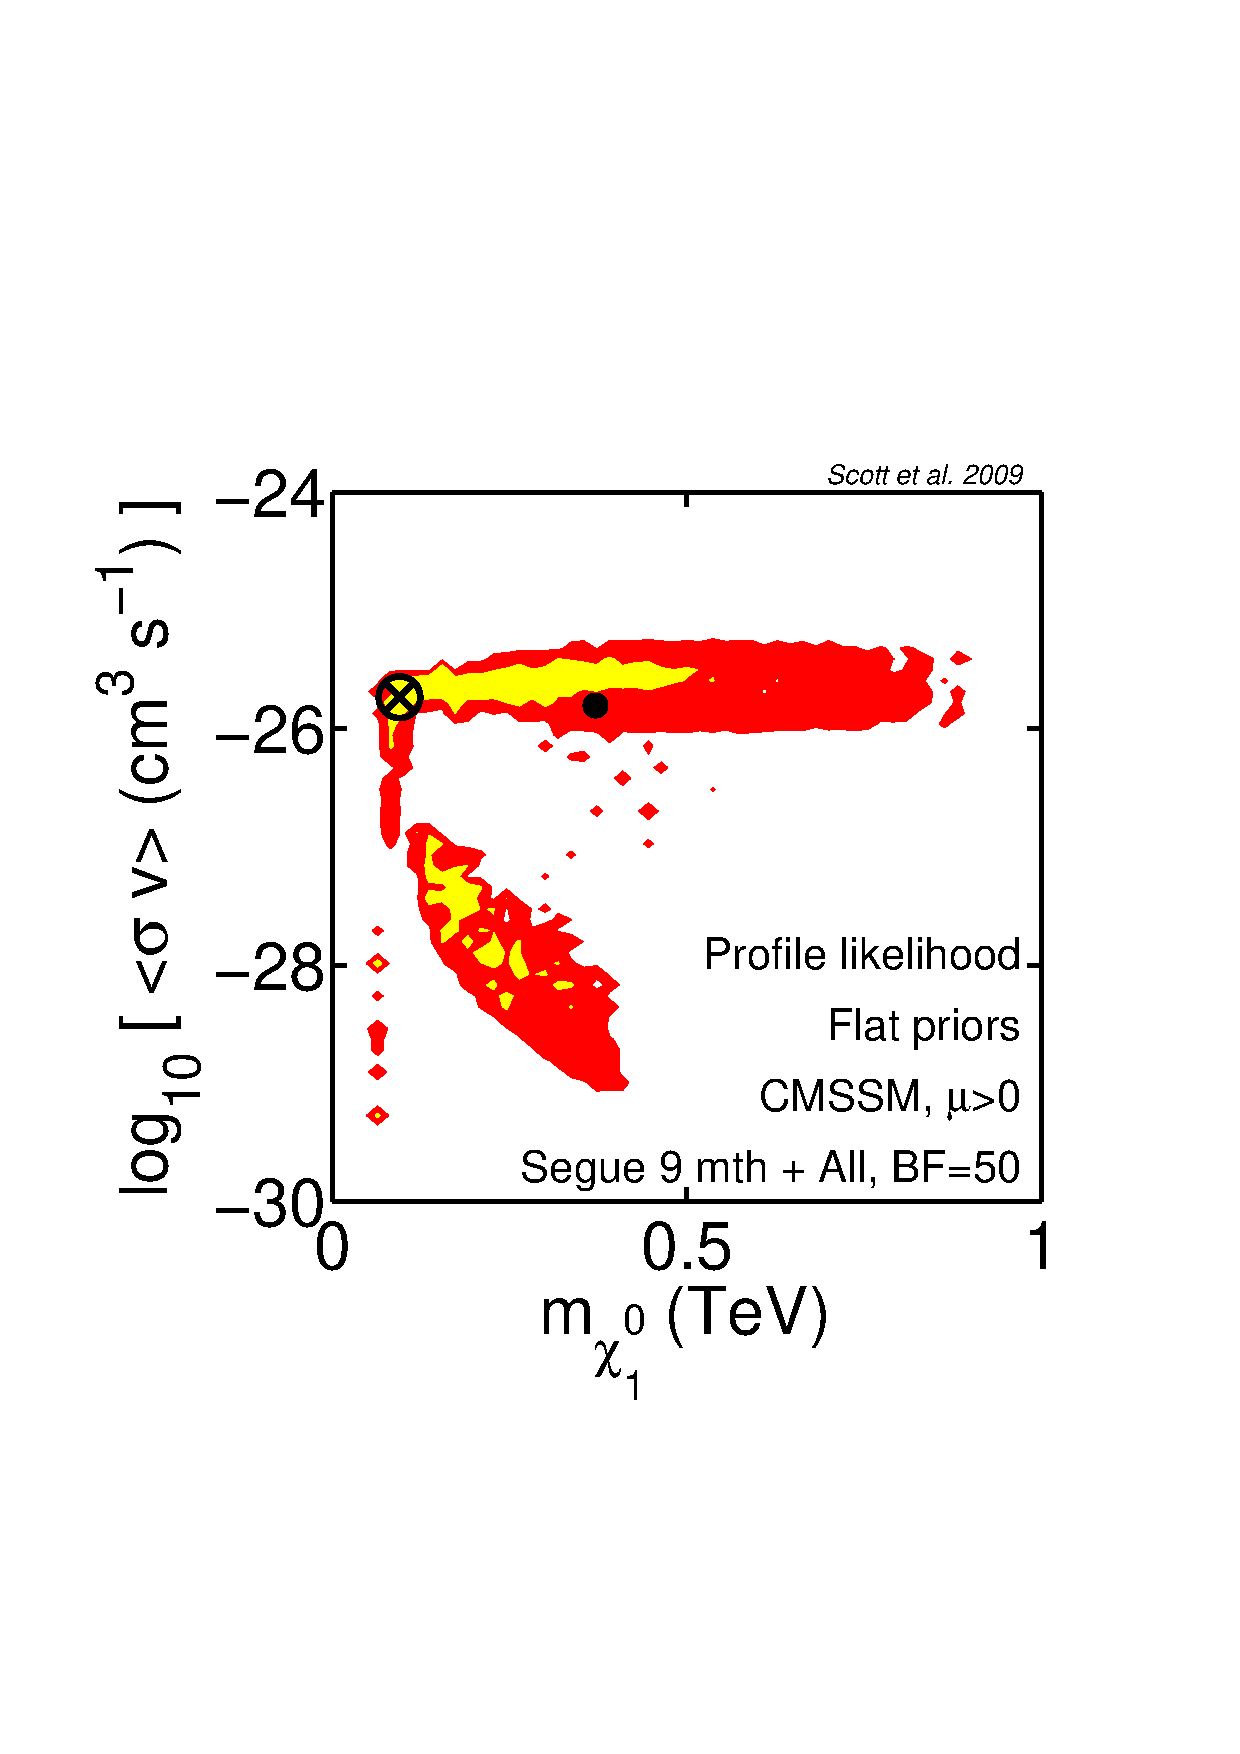
\includegraphics[height=0.6\textwidth, trim = 20 182 20 220, clip=true]{B50_H0_All_P_lin_2D_profl_7}}%
\only<3>{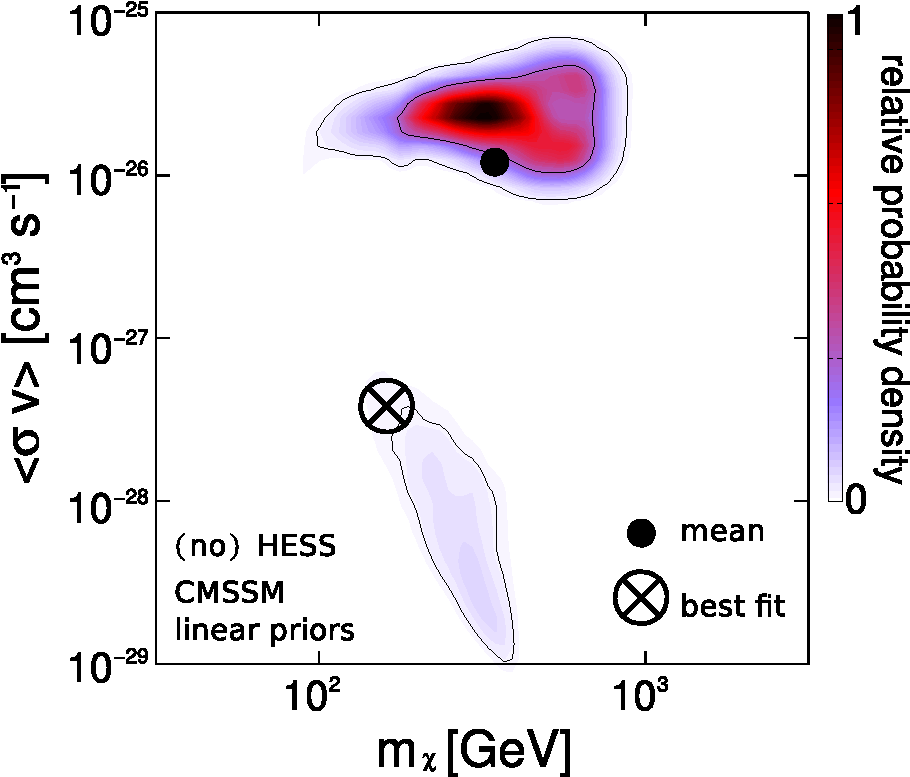
\includegraphics[height=0.6\textwidth]{noHESS}}%
\only<4>{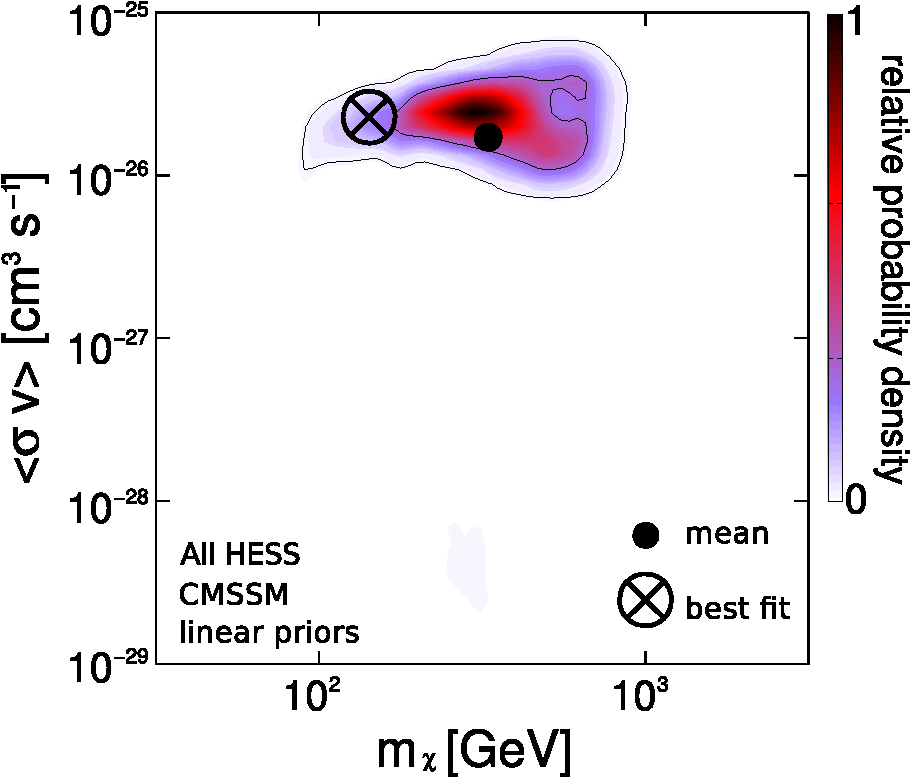
\includegraphics[height=0.6\textwidth]{allHESS}}

\column{0.6\linewidth}
\only<1>{\footnotesize\vspace{-3mm}
\begin{itemize}
\item Full binned Poissonian likelihood (no $\chi^2$ approximation)
\item Full treatment of PSF \textit{and} energy dispersion (with fast convolution library FLATlib) 
\item Marginalisation over systematic error on effective area
\item Diffuse BG from Fermi-LAT Galprop fits
\item Isotropic BG best-fit isotropic power law
\item $J$-factor from Martinez et al (\textit{JCAP}, 0902.4715; best at the time)
\end{itemize}
}%
\only<2>{\footnotesize
The other notable effort in this vein:\\ combined dwarf pMSSM random scan by Cotta et al \textit{JCAP}, 1111.2604
}%
\only<4>{
\begin{itemize}
\item $\chi^2$-based analysis using public flux limits
\item `Milky Way' = halo just beyond GC (45--150\,pc)
\item Virtual internal bremsstrahlung from co-annihilation strip models caught at high-$E$ by HESS 
\item but: $J$-factors for Sag dwarf rather uncertain

\end{itemize}
}

\end{columns}

\end{frame}


\subsection{Neutrinos}

\begin{frame}
\frametitle{Example: Advanced IceCube Likelihood (Part 1)}

Simplest way to do anything is to make it a counting problem\ldots

\vspace{5mm}

Compare observed number of events $n$ and predicted number $\theta$ for each model, taking into account error $\sigma_\epsilon$ on acceptance:

\begin{equation}
\label{fancy}
\scriptsize
\Like_\mathrm{num}(n|\theta_\mathrm{BG}+\theta_\mathrm{sig}) = \frac{1}{\sqrt{2\pi}\sigma_\epsilon}\int_0^\infty \frac{(\theta_\mathrm{BG}+\epsilon\theta_\mathrm{sig})^{n}e^{-(\theta_\mathrm{BG}+\epsilon\theta_\mathrm{sig})}}{n!}\frac1\epsilon\exp\left[-\frac{1}{2}\left(\frac{\ln\epsilon}{\sigma_\epsilon}\right)^2\right]\mathrm{d}\epsilon \, .
\end{equation}
\vspace{3mm}

Nuisance parameter $\epsilon$ takes into account systematic errors on effective area, from theory, etc.  $\sigma_\epsilon\sim20\%$ for IceCube.



\end{frame}



\begin{frame}

\frametitle{Example: Advanced IceCube Likelihood (Part 2)}
Full unbinned likelihood with number ($\Like_\mathrm{num}$), spectral ($\Like_\mathrm{spec}$) and angular ($\Like_\mathrm{ang}$) parts 
\begin{equation}
\footnotesize
\Like = \Like_\mathrm{num}(n|\theta_{\mathrm{signal+BG}})\prod_{i=1}^{n} \Like_{\mathrm{spec},i}\,\Like_{\mathrm{ang},i}
\end{equation}
with
\begin{equation}
\footnotesize
\Like_{\mathrm{spec},i}(\alert<2-3>{N_i}, \corangewhen{\params}{<3>}) = \frac{\theta_\mathrm{BG}}{\theta_\mathrm{signal+BG}}\cgreenwhen{\frac{dP_\mathrm{BG}}{d\alert<2-3>{N_i}}(\alert<2-3>{N_i})}{<6>} +\frac{\theta_\mathrm{signal}}{\theta_\mathrm{signal+BG}}\int_0^\infty \corangewhen{E_\mathrm{disp}(\alert<2-3>{N_i}|\Eobsi)}{<5-6>}\cbluewhen{\frac{dP_\mathrm{signal}}{d\Eobsi}(\Eobsi, \corangewhen{\params}{<3>})}{<4-6>} \,d \Eobsi
\end{equation}
and
\begin{equation}
\footnotesize
\Like_{\mathrm{ang},i}(\cgreenwhen{\cos\phi_i}{<7>}) = \frac{\theta_\mathrm{BG}}{\theta_\mathrm{signal+BG}}\cgreenwhen{\frac{dP_\mathrm{BG}}{d\cgreenwhen{\cos\phi_i}{<7>}}(\cgreenwhen{\cos\phi_i}{<7>})}{<10>} + \frac{\theta_\mathrm{signal}}{\theta_\mathrm{signal+BG}}\corangewhen{PSF(\cgreenwhen{\cos\phi_i}{<7>}|\cbluewhen{1}{<8-10>})}{<9-10>}
\end{equation}

\only<2-3>{
\begin{textblock}{80}(20,46)
\alert{Number of lit channels (energy estimator)}
\end{textblock}
}
\only<3>{
\begin{textblock}{40}(70,61)
\corange{BSM theory parameters}
\end{textblock}
}
\only<4-6>{
\begin{textblock}{80}(50,44)
\cblue{Predicted signal spectrum (from theory)}
\end{textblock}
}
\only<5-6,9-10>{
\begin{textblock}{60}(70,61)
\corange{Instrument response function}
\end{textblock}
}
\only<6,10>{
\begin{textblock}{60}(25,61)
\cgreen{Observed BG distribution}
\end{textblock}
}
\only<7>{
\begin{textblock}{40}(20,76)
\cgreen{Event arrival angle}
\end{textblock}
}
\only<8-10>{
\begin{textblock}{80}(40,76)
\cblue{Predicted signal direction ($\delta$ function at Sun)}
\end{textblock}
}
\end{frame}

\begin{frame}
\frametitle{Global fits with IceCube event data}

New likelihood analysis including IceCube Neutrino Telescope WIMP-search neutrino events
\vspace{3mm}

\begin{columns}[t]
\column{0.58\linewidth}
\visible<1-4>{%
  \cblue{IceCube 22-string data}\\
  {\footnotesize
    Not expected to be very constraining\\
    \visible<2-4>{\ldots but at least we know it works}\\
    {\tiny(PS, Savage, Edsj\"o \& IceCube {\it JCAP}, 1207.0810)}
    \only<1,3-4>{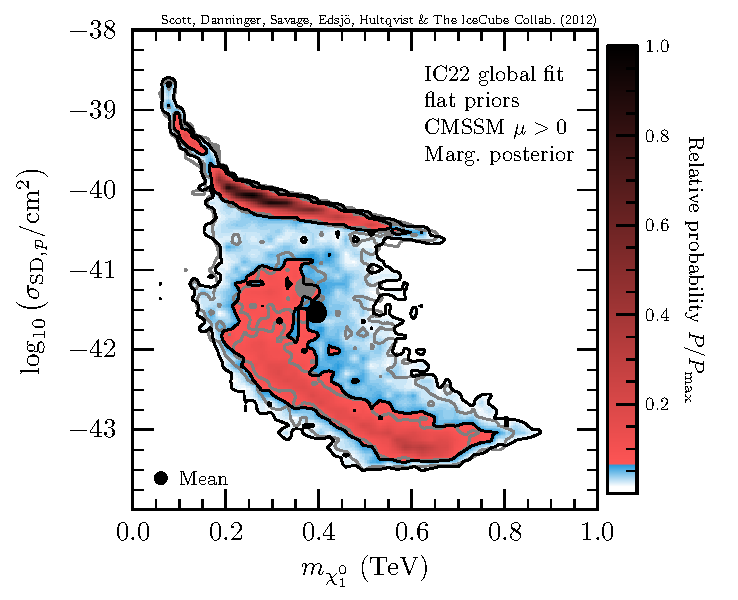
\includegraphics[width=0.85\textwidth]{IC22_marg3}}%
    \only<2,5>{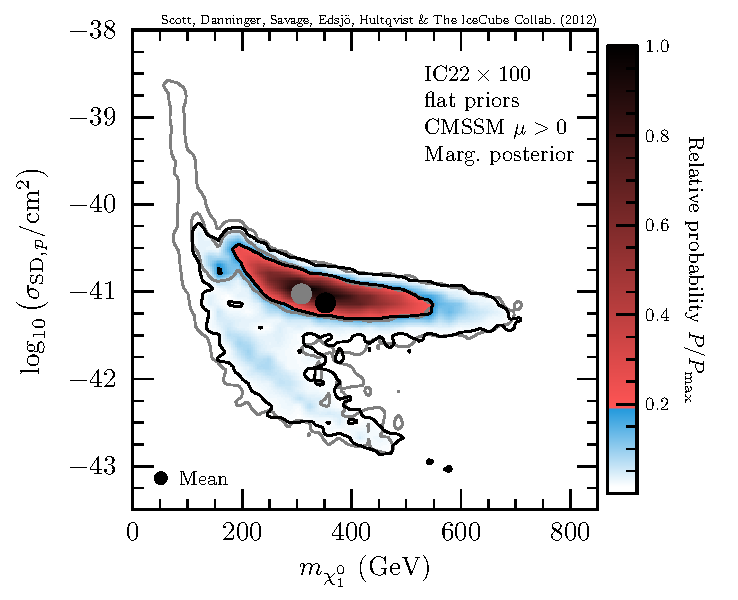
\includegraphics[width=0.85\textwidth]{recon2D_4}}
  }%
}

\column{0.58\linewidth}
\visible<1-4>{%
  \visible<3-4>{%
    \cblue{IceCube-DeepCore (86-string)}\\
    {\footnotesize%
      Very constraining (projection)%
      \visible<4>{%
        $\implies$ unique access to pts in more general MSSM\\
        {\tiny(Silverwood, PS, Danninger et al {\it JCAP}, 1210.0844)}}
    }%
  }%
}
\only<2>{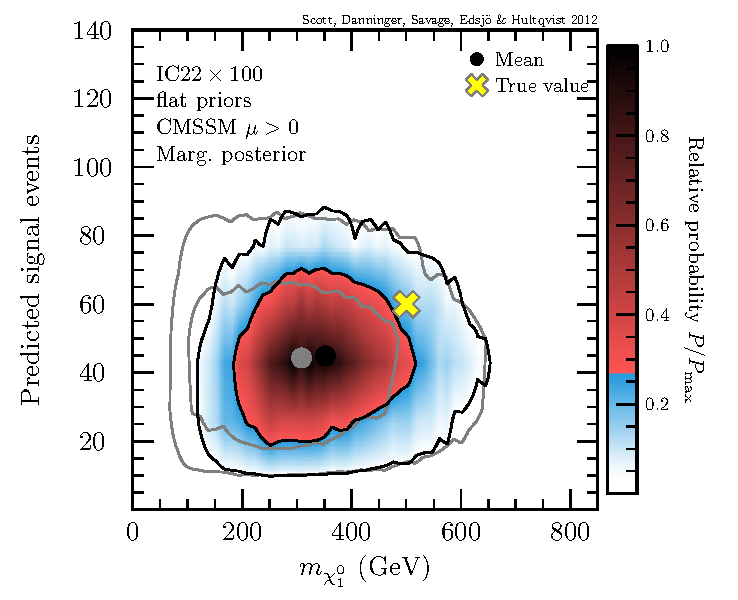
\includegraphics[width=0.85\textwidth]{recon2D_5}}%
\only<3>{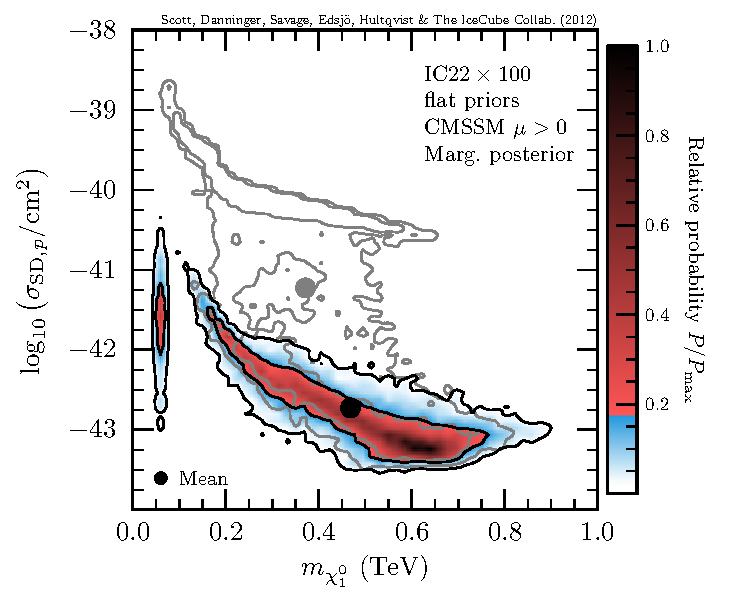
\includegraphics[width=0.85\textwidth]{IC22x100_marg3}}%
\only<4>{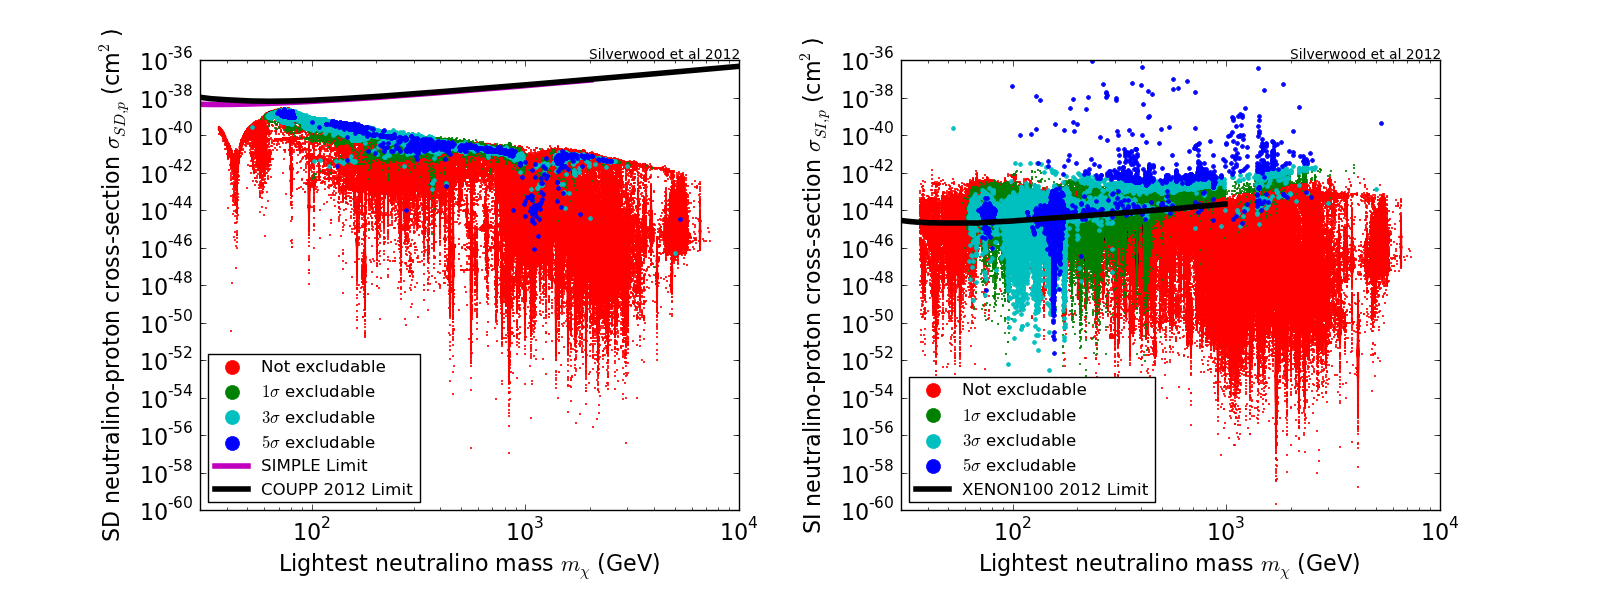
\includegraphics[width=0.9\textwidth, trim = 550 0 0 0, clip=true]{MSSM25}}
\end{columns}


\only<5>{
\begin{textblock}{90}(15,35)
The examples here are CMSSM \& MSSM-25 -- but this about a framework, applicable to any model.  
\vspace{3mm}

{\alert{All the methods discussed here are available in DarkSUSY v5.0.6 and later: }{\color[rgb]{0.1, 0.0, 0.6}\href{www.darksusy.org}{www.darksusy.org}}
\vspace{3mm}}

{All IceCube data used are available at {\color[rgb]{0.1, 0.0, 0.6}\href{http://icecube.wisc.edu/science/data/ic22-solar-wimp}{http://icecube.wisc.edu/science/data/ic22-solar-wimp}} (and in DarkSUSY, for convenience)}\\
\end{textblock}

}

\end{frame}


\begin{frame}
\frametitle{Example of Combined Direct + Indirect + LHC constraints}

\Large

\visible<1-4>{Base Observables} \visible<2-4>{$+$ XENON-100}\only<2>{ (2011)} \only<3-4>{$+$ CMS\,5\,fb$^{-1}$}

{\centering \visible<4>{$+$ IC22$\times$100}}

\vspace{2mm}
\footnotesize
\visible<2-4>{Grey contours correspond to Base Observables \textit{only}}
\vspace{2mm}

\begin{columns}
\column{0.36\textwidth}
\only<1>{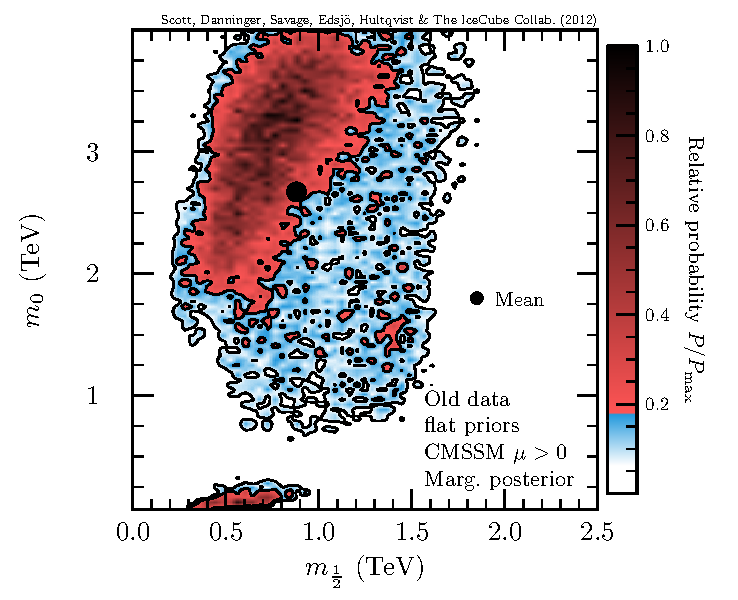
\includegraphics[height=0.92\linewidth, trim = 8 0 30 0, clip = true]{marg2D_1_1}}%
\only<2>{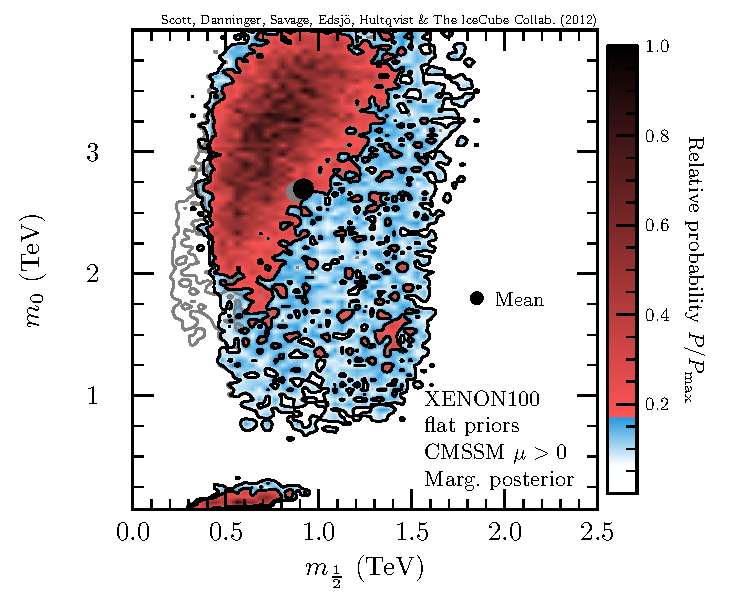
\includegraphics[height=0.92\linewidth, trim = 8 0 30 0, clip = true]{marg2D_2_1}}%
\only<3>{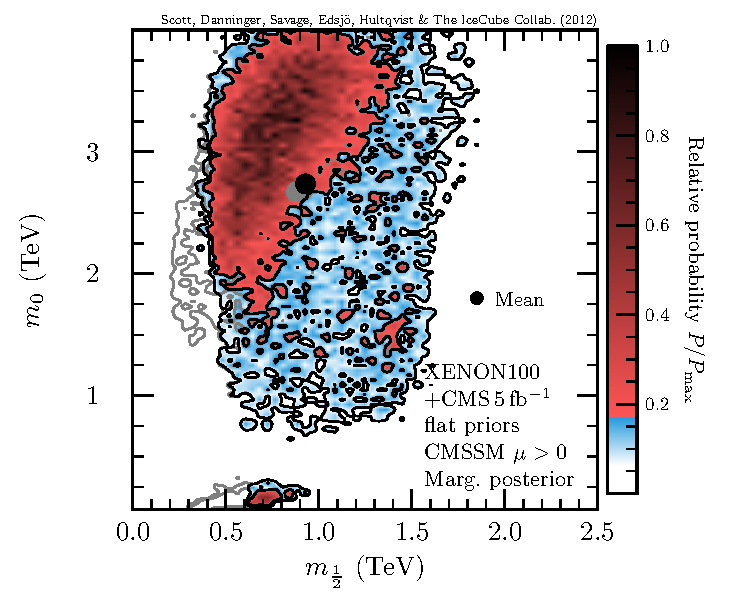
\includegraphics[height=0.92\linewidth, trim = 8 0 30 0, clip = true]{marg2D_3_1}}%
\only<4>{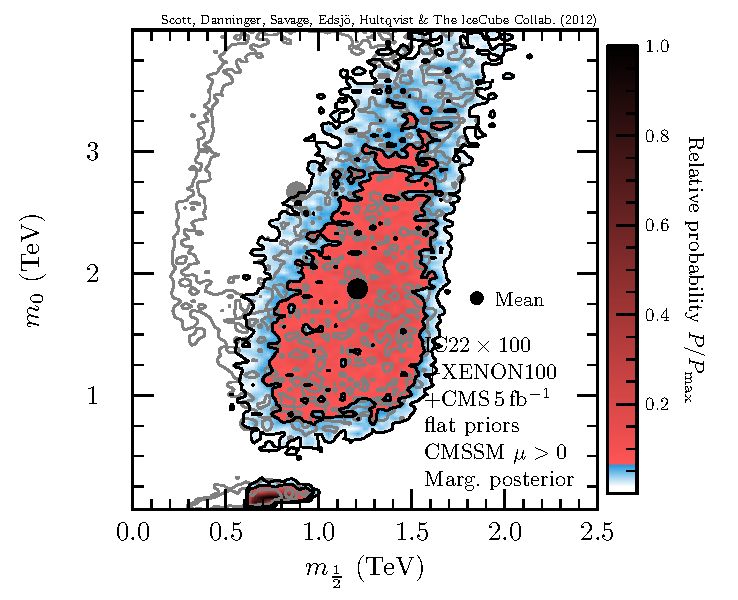
\includegraphics[height=0.92\linewidth, trim = 8 0 30 0, clip = true]{marg2D_4_1}}
\column{0.36\textwidth}
\only<1>{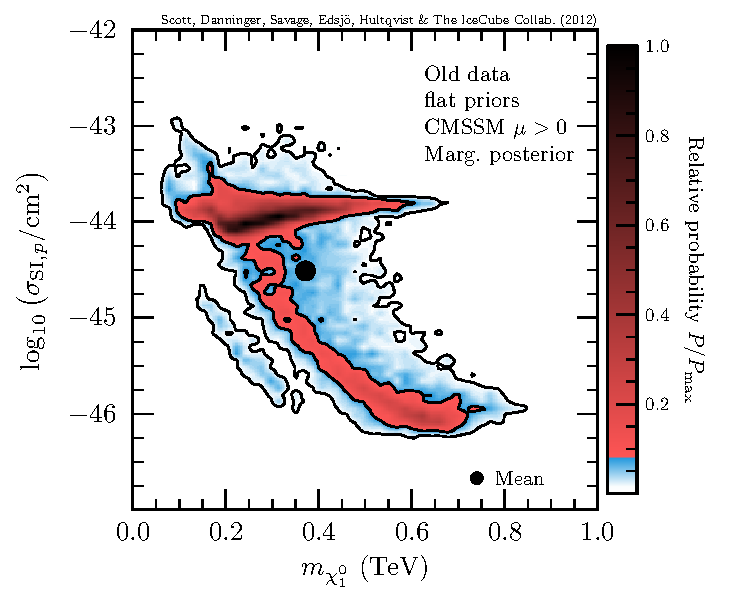
\includegraphics[height=0.92\linewidth, trim = 8 0 30 0, clip = true]{marg2D_1_2}}%
\only<2>{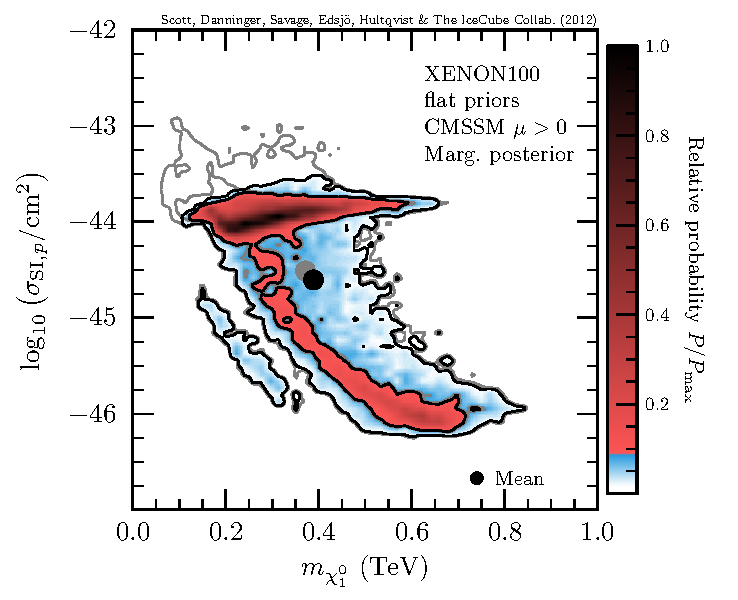
\includegraphics[height=0.92\linewidth, trim = 8 0 30 0, clip = true]{marg2D_2_2}}%
\only<3>{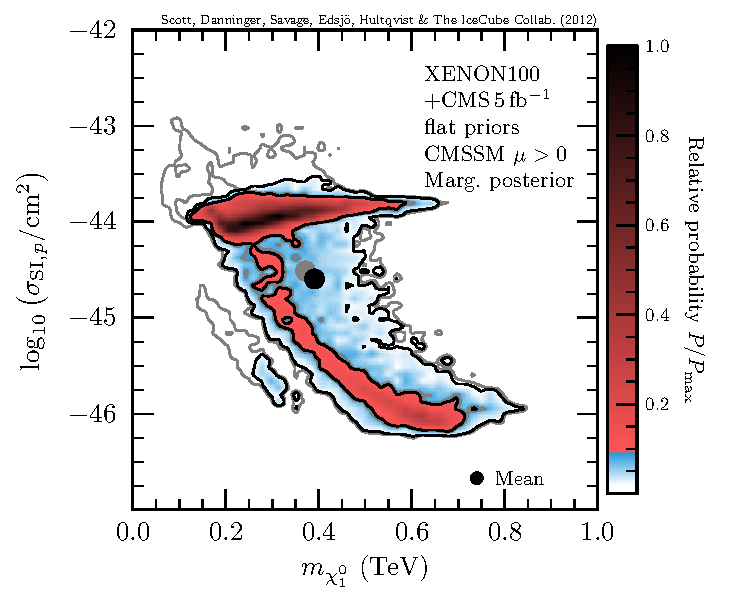
\includegraphics[height=0.92\linewidth, trim = 8 0 30 0, clip = true]{marg2D_3_2}}%
\only<4>{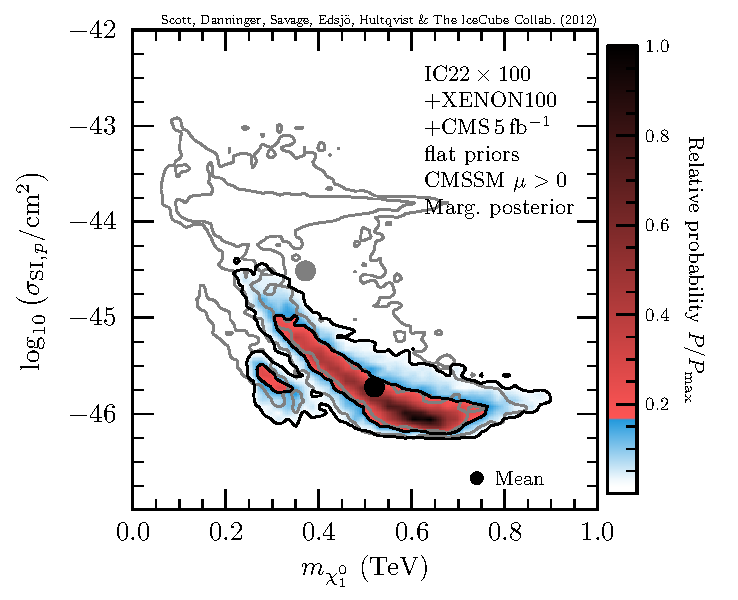
\includegraphics[height=0.92\linewidth, trim = 8 0 30 0, clip = true]{marg2D_4_2}}
\column{0.36\textwidth}
\only<1>{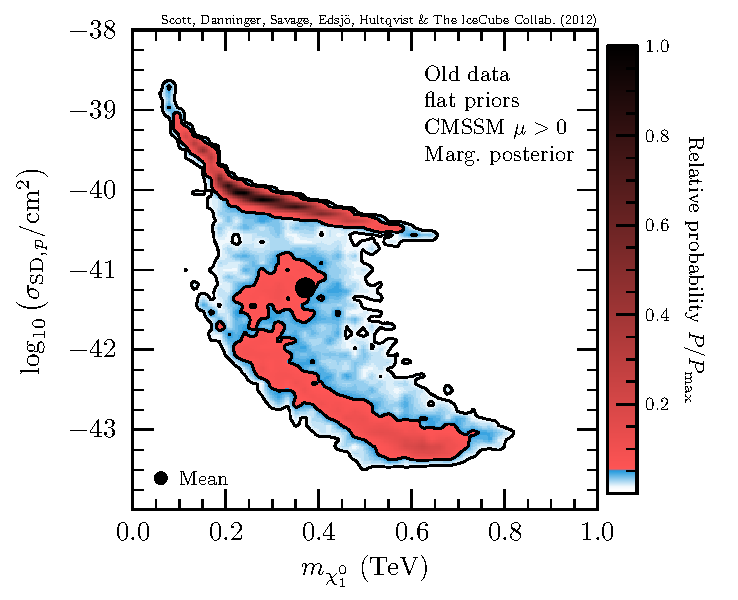
\includegraphics[height=0.92\linewidth, trim = 8 0 10 0, clip = true]{marg2D_1_3}}%
\only<2>{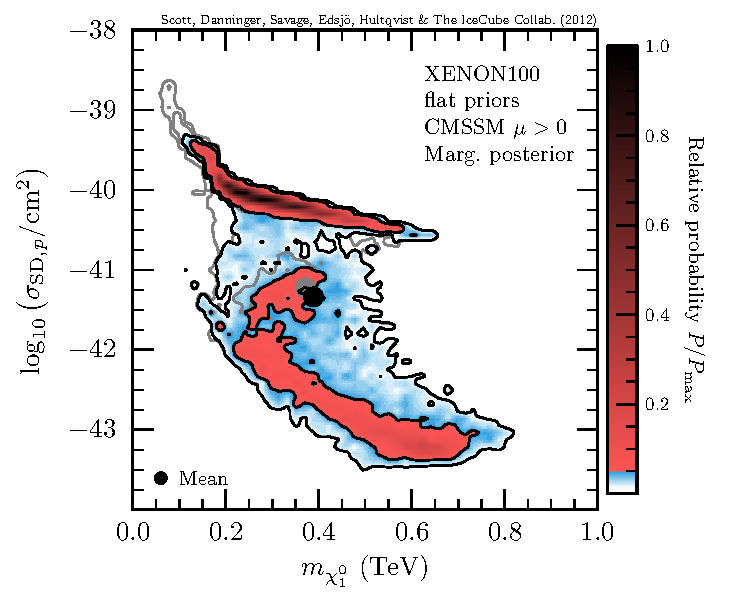
\includegraphics[height=0.92\linewidth, trim = 8 0 10 0, clip = true]{marg2D_2_3}}%
\only<3>{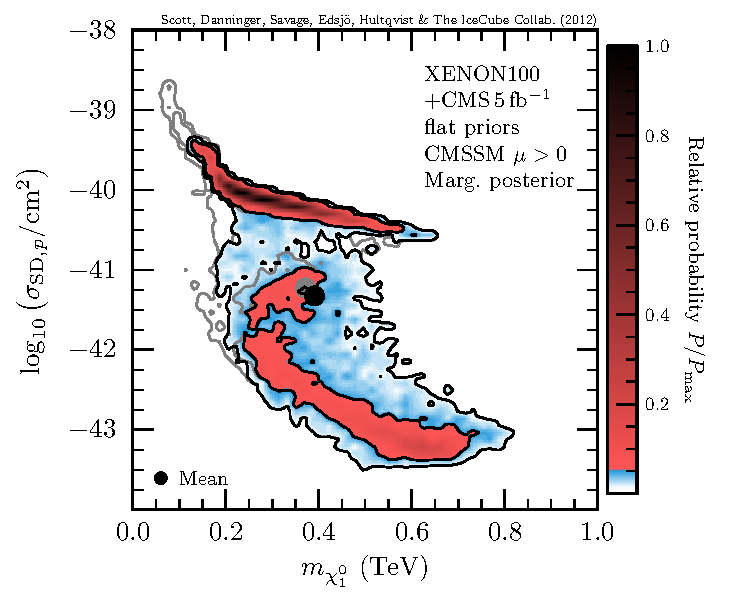
\includegraphics[height=0.92\linewidth, trim = 8 0 10 0, clip = true]{marg2D_3_3}}%
\only<4>{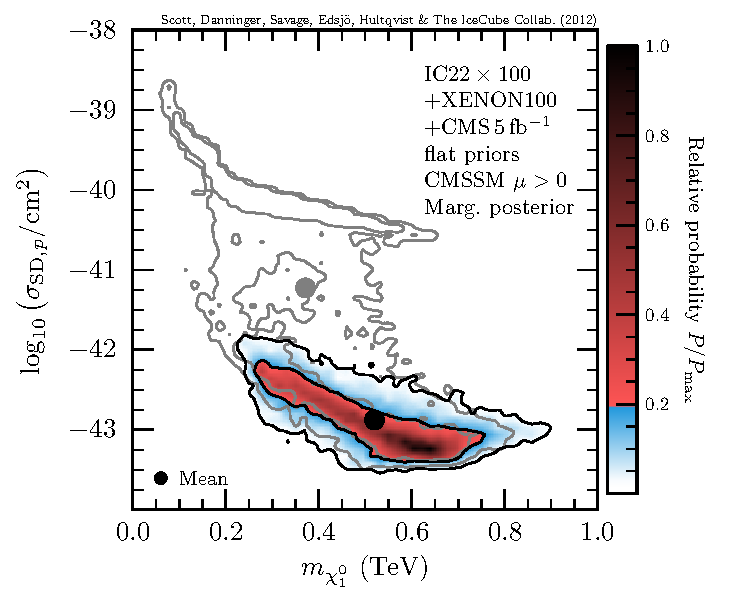
\includegraphics[height=0.92\linewidth, trim = 8 0 10 0, clip = true]{marg2D_4_3}}
\end{columns}
\vspace{2mm}

\visible<4>{\textbf{CMSSM, IceCube-22 with 100$\times$ boosted effective area}\\
(kinda like IceCube-DeepCore)}

\end{frame}

\subsection{CMB constraints}

\begin{frame}
\frametitle{Generalised DM CMB likelihood functions}

Simple CMB likelihood function, for
\begin{itemize}
\item Any combination of annihilation or decay channels
\item Any dark matter mass 
\item Any decay lifetime/annihilation cross-section
\end{itemize}
$\rightarrow$ just requires interpolating one number in a table.\vspace{5mm}

\visible<2-3>{
$f_\mathrm{eff}$ for annihilation:
\begin{equation}\footnotesize
 \ln\,\mathcal{L}(\langle\sigma v\rangle|m_\chi,r_i) = -\frac12 f_{\rm eff}^2(m_\chi,r_i) \lambda_1 c_1^2\,
 \left(\frac{\langle\sigma v\rangle}{2\times 10^{-27}{\rm cm}^3{\rm s}^{-1}}\right)^2\,\left(\frac{\rm GeV}{m_\chi}\right)^2
\label{loglike2}
\end{equation}
}

\visible<3>{
$\eta$ for decay:
\begin{equation}\footnotesize
\ln\, \mathcal{L}(\tau|m_\chi,r_i) = -\frac12\left(\delta\Omega\over\Omega_\mathrm{DM}\tau\right)^2\eta^2(\tau,m_\chi,r_i)
\end{equation}
}


\begin{textblock}{70}(15,48)
  \visible<4>{
    \begin{columns}
    \column{0.6\linewidth}
    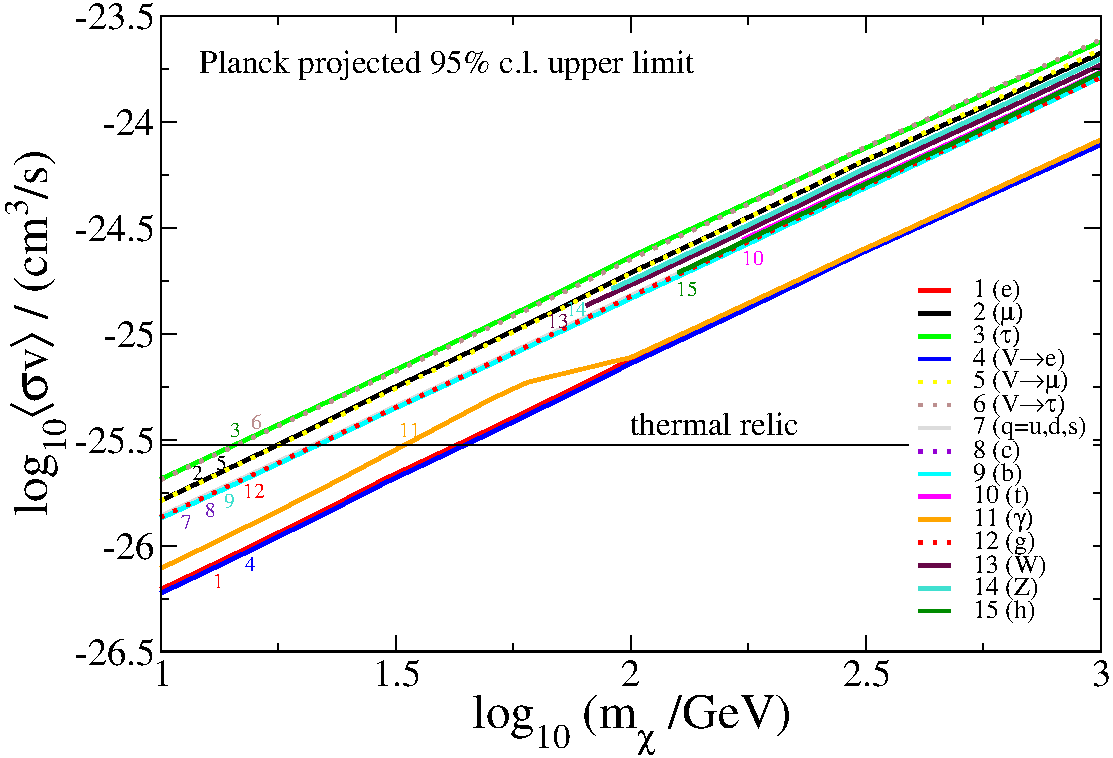
\includegraphics[width=1.1\textwidth]{planck-limit}
    \column{0.1\linewidth}
    \column{0.6\linewidth}
    \includegraphics[width=1.1\textwidth]{electrons-w-planck}
    \end{columns}
  }
\end{textblock}

\begin{textblock}{80}(15,49)
  \visible<1>{
  Cline \& PS, 1301.5908, using
  \begin{itemize}
    \item CMB energy deposition from Slatyer, 1211.0283 and Finkbeiner et al, 1109.6322
    \item PYTHIA annihilation/decay spectra of Cirelli et al, 1012.4515.
  \end{itemize}
  }
\end{textblock}

\end{frame}

\section{Future Challenges}

\subsection{Respectable LHC likelihoods}

\begin{frame}
\frametitle{The LHC likelihood monster}

\visible<1->{
\begin{exampleblock}{Time per point:}
$\mathcal{O}(minute)$ in \alert{best} cases
\end{exampleblock}
}

\visible<2->{
\begin{exampleblock}{Time per point for global fits to converge:}
$\mathcal{O}(seconds)$ in \alert{worst} cases
\end{exampleblock}
}

\visible<3->{
\begin{exampleblock}{Challenge:}
About 2 orders of magnitude too slow to actually include LHC data in global fits properly
\end{exampleblock}
}

\end{frame}

\begin{frame}
\frametitle{Taming the LHC monster}

\only<1,2>{
\begin{exampleblock}{Zeroth Order Response:}
``Stuff it, just use the published limits and ignore the dependence on other parameters''
\end{exampleblock}

\visible<2>{
\vspace{5mm}
Obviously naughty -- plotted limits assume CMSSM, and fix two of the parameters
\begin{itemize}    
  \item Don't really know dependence on other parameters
  \item Don't have a likelihood function, just a line
  \item Can't use this at all for non-CMSSM global fits -- e.g. MSSM-25
\end{itemize}
}}  

\only<3,4>{
\begin{exampleblock}{First Order Response:}
``Test if things depend on the other parameters (hope not), re-simulate published exclusion curve''
\end{exampleblock}

\visible<4>{
\vspace{5mm}
Not that great, but OK in some cases
\begin{itemize}    
  \item At least have some sort of likelihood this time
  \item Still a bit screwed if things do depend a lot on other parameters, but
  \item allows (potentially shaky) extrapolation, also to non-CMSSM models
\end{itemize}

\vspace{5mm}
Fittino, Mastercode
}}

\only<5,6>{
\begin{exampleblock}{Second Order Response:}
``That's ridiculous.  I've never met a calculation I can't speed up.  There must be some way to have my cake and eat it too''
\end{exampleblock}

\visible<6>{
\vspace{5mm}
Maybe -- this is the challenge.
\begin{itemize}    
  \item Interpolated likelihoods (how to choose nodes?)
  \item Neural network functional approximation (how to train accurately?)
  \item Some sort of smart reduction based on event topology? 
  \item Something else?
\end{itemize}
}}

\end{frame}


\subsection{Coverage \& optimisation vs contour mapping}

\cblue{We don't \textit{*really*} know the distribution of our test statistic in BSM global fits, as it is too expensive to Monte Carlo}
      \begin{itemize}\footnotesize
                 \item coverage is rarely spot-on unless mapping from parameters to data-space is linear \\
                 {\tiny(Akrami, Savage, PS et al {\it JCAP}, 1011.4297, Bridges et al {\it JHEP}, 1011.4306, Strege et al {\it PRD}, 1201.3631)}
                 \item $p$-value assessments of goodness of fit should be viewed with scepticism ($\rightarrow$MasterCode)
                 \end{itemize}
\cblue{Convergence remains an issue, especially for profile likelihood}\\
Messy likelihood $\implies$ best-fit point can be (and often is) easily missed {\tiny(Akrami, PS et al {\it JHEP}, 0910.3950, Feroz et al {\it JHEP}, 1101.3296)}
      \begin{itemize}\footnotesize
                 \item frequentist CLs are often off, as isolikelihood levels are chosen incorrectly
                 \item can impact coverage (overcoverage, or masking of undercoverage due to non-$\chi^2$ $TS$ distribution)
                 \item need to use multiple priors and scanning algorithms (one optimised for profile likelihoods?)  
                 \end{itemize}


\subsection{Parameter space $\rightarrow$ Theory space}

\begin{frame}
\frametitle{CMSSM, SMS $\ne$ BSM}

(SMS = Simplified Model Spectrum)
\vspace{3mm}

Want to do model comparison to actually work out which theory is right\ldots
\vspace{3mm}

\begin{exampleblock}{Challenge:}
How do I easily adapt a global fit to different BSM theories?
\end{exampleblock}

\visible<2>{
Somehow, we must recast things quickly to a new theory 
\begin{itemize}
\item data
\item likelihood functions
\item scanning code `housekeeping'
\item even predictions
\end{itemize}
$\implies$ a new, very abstract global fitting framework
}

\end{frame}

\begin{frame}
\frametitle{Hitting the wall}

Issues with current global fit codes:
\begin{itemize}
\item Strongly wedded to a few theories (e.g. constrained MSSM / mSUGRA)
\item Strongly wedded to a few theory calculators
\item All datasets and observables basically hardcoded
\item Rough or non-existent treatment of most experiments (astroparticle + collider especially)
\item Sub-optimal statistical methods / search algorithms
\item $\implies$ \textit{already hitting the wall on theories, data \& computational methods}
\end{itemize}

\end{frame}

\begin{frame}
\frametitle{\textbf{GAMBIT}: a \textit{second-generation} global fit code}

GAMBIT: \alert{G}lobal \alert{A}nd \alert{M}odular \alert{B}SM \alert{I}nference \alert{T}ool
\vspace{5mm}

Overriding principles of GAMBIT: flexibility and modularity
\begin{itemize}
\item General enough to allow fast definition of new datasets and theoretical models
\item Plug and play scanning, physics and likelihood packages
\item Extensive model database -- not just small modifications to constrained MSSM (NUHM, etc), and not just SUSY!
\item Extensive observable/data libraries (likelihood modules)
\item Many statistical options -- Bayesian/frequentist, likelihood definitions, scanning algorithms
\item A smart and \textit{fast} LHC likelihood calculator
\item Massively parallel
\item Full open-source code release
\end{itemize}

\end{frame}


\begin{frame}
\frametitle{The GAMBIT Collaboration}

23 Members, 12 Institutes \\
8 Experiments, 3 major theory codes \vspace{3mm}

\begin{tabular}{l l}
\textbf{Fermi-LAT} & \small J.\ Conrad, J.\ Edsj\"o, G.\ Martinez, P.\ Scott {\tiny(Coordinator)}\\
\textbf{IceCube} & \small J.\ Edsj\"o, C.\ Savage, P.\ Scott\\
\textbf{ATLAS} & \small A.\ Buckley, C.\ Clement, P.\ Jackson, A.\ Saavedra, M.\ White\\
\textbf{CMS} & \small C.\ Rogan\\
\textbf{HESS} & \small J.\ Conrad, H.\ Dickinson \\
\textbf{AMS-02} & \small A.\ Putze\\
\textbf{CTA} & \small T.\ Bringmann, J.\ Conrad, H.\ Dickinson\\
\textbf{DARWIN} & \small J.\ Conrad\\
\textbf{Theory} & \small C. Bal\'azs, T.\ Bringmann, L.-A.\ Dal, J.\ Edsj\"o, \\
                & \small B.\ Farmer, A.\ Krislock, A.\ Kvellestad, N.\ Mahmoudi, \\
                & \small A.\ Raklev, C.\ Savage, P.\ Scott, C.\ Weniger \\	
\end{tabular}

\end{frame}


\begin{frame}
\frametitle{Closing remarks}

\begin{itemize}
\item{Robust analysis of dark matter and BSM physics requires multi-messenger global fits}
\item{Lots of interesting astroparticle observables to include in global fits}
\item{Quite a bit of technical (statistical/computational) detail to worry about}
\item{GAMBIT is coming}
\end{itemize}


\end{frame}

\end{document}




